%==========================================================================
% BEGIN #1 - INTRO
% Apresentação geral do trabalho que se pretende realizar, bem como revelar a forma como ele se irá desenvolver (ou desenvolveu) ao longo do tempo que têm para o fazer.
%==========================================================================


\chapter{Introdução}
    
    \section{Contextualização}
        
        O empresário António Silva Faria, sendo um entusiasta, colecionador e artista LEGO de longa data, considerou oportuno abrir um negócio de montagem de modelos, com maior ênfase nos modelos expositivos. 
        
        Assim, fundou-se a BlocoPronto Lda, operando segundo mail-order centralizada.
        
        A empresa foi bem-vinda na comunidade, de tal modo que a afluência de pedidos levou ao desenvolvimento do, inicialmente, pequeno negócio para grande escala.

    \section{Apresentação do Caso de Estudo}
        
        De modo ineficaz, a comunicação na empresa era totalmente feita por correio eletrónico, quer entre o cliente e a empresa (encomenda; aceitação/rejeição; faturação; apoio e esclarecimento), quer entre a empresa e o fornecedor (reposições de inventário).


        O representante pela comunicação recebe uma encomenda, que teria de encaminhar para o coordenador da linha de montagem, este teria que verificaria o stock e a viabilidade da conceção da encomenda, após isto iria reponder ao representante se seria possível concretizar a encomenda. Só após este processo, totalmente à mercê da habilidade logística de dois encarregados de áreas distintas, é que o cliente saberia se a encomenda seria realizada ou não. Para um coordenador da linha de montagem verificar esta viabilidade, seria necessária uma consulta da lista de peças necessárias, obtida no \textit{website} oficial LEGO, e confrontá-la com o inventário disponível.
        
    \newpage
    \section{Motivação e Objectivos}
        
        Com o passar do tempo, a procura pela empresa cresceu consideravelmente. Com este crescimento tornou-se evidente que a logística da empresa não era eficaz: havia um volume absurdo de emails e frequência das consultas comparativamente à quantidade de encomendas efetivamente concebidas - um calcanhar de Aquiles na escalabilidade e no \textit{throughput} das linhas de montagem. Claro se torna que isto se deve ao facto de a empresa depender de plataformas que não foram desenvolvidas para o uso que estão a ter. Problema que a administração quer resolver.


        Em média, funcionários das empresas com cargo interativo ocupam cerca de 28\% e 20\% do seu tempo laboral na gestão de emails e na busca por informação interna, respetivamente\cite{Chui2012}. No caso da BlocoPronto, segundo análises internas do ano anterior, estes valores são 39\% e 26\%, respetivamente, o que fez suscitar a vontade de criar uma plataforma adaptada às necessidades logísticas da empresa, que permitisse alocar mais tempo para a montagem. Com isto em mente, a nova plataforma disponibilizaria, de forma unificada:

        \begin{enumerate}
            \item Consulta a Referências dos Modelos LEGO
            \begin{itemize}
                \item Armazenamento interno dos manuais instrucionais;
                \item Visualização passo-a-passo das etapas de montagem na linha.
            \end{itemize}

            \item Gestão sobre Encomendas de Montagem
            \begin{itemize}
                \item Listagem de encomendas pendentes à medida que chegam;
                \item Teste automático da viabilidade de conceção da encomenda segundo o inventário;
                \item Processamento (aceitação/rejeição) da encomenda segundo a viabilidade;
                \item Ordenação em fila das encomendas a conceber.
            \end{itemize}
        
            \item Manutenção de Inventário
            \begin{itemize}
                \item Listagem das peças atualmente disponíveis e em que respetivas quantidades;
                \item Criação de pedidos para reposição de inventário.
            \end{itemize}
        \end{enumerate}

    \newpage
    \section{Estrutura do Relatório}
    
        O desenvolvimento do sistema conta com - até ao momento de publicação - cinco fases, cada qual correspondente a um capítulo no índice. Eis uma curta descrição do que cada uma aborda:
    
        \begin{enumerate}
            \item Reflete sobre o contexto fundamental (a razão de ser) do sistema, o que colmataria (e como, de grosso modo) e o que implicaria em recursos e logística.
            \item Revela a estipulação final dos requisitos do sistema e, adicionalmente, relata-se a estratégia que a equipa encarregada usou, dentro do contexto da hipotética empresa, para os obter.
            \item Com base nos requisitos, apresentam-se os modelos e especificações geradas, em registo conceptual e corrente, para ajudar à definição da arquitetura e do comportamento sob utilização.
            \item É definida e explicada uma estrutura concreta para a camada de dados.
            \item Expõem-se esboços da interface gráfica, tais estes que também serviriam de material a expôr ao cliente hipotético.
        \end{enumerate}

    O capítulo 6 dá como concluída esta primeira metade do desenvolvimento com uma crítica retrospetiva das suas fases e um comentário sobre a metade seguinte.   

    \newpage
    \section{Justificação e Utilidade do Sistema}
        O sistema vem colmatar as barreiras impostas às montagens e o atraso na sua iniciação causados pela necessidade de confirmação humana para responder a encomendas e pelo uso de plataformas disjuntas e inadaptadas. Este vem também permitir um aumento da frequência e velocidade de resposta a pedidos de montagem e, consequentemente, de modelos montados e eficiência laboral.

        
        Dum modo sucinto, sentir-se-ão os seguintes efeitos na empresa:
        \begin{itemize}
            \item Aumento da parcela temporal que os montadores usam para efetivamente montar durante o horário de trabalho, dado o fluxo mais conveniente e automatizado que se introduz;
            
            \item Redução da dependência inter-departamento de cariz substituível por registos elaborados por máquina;
            
            \item Melhoria da reputação com os clientes, desprendendo o representante das funções notificáveis diretamente pela produção, este torna-se mais flexível para relações públicas;
            
            \item Aumento da quantidade de modelos montados por dia;
            
            \item Aceleração do processo de integração de novos montadores, vista a simplificação do fluxo das diferentes tarefas inerentes ao cargo.
        \end{itemize}
        
        Tendo em consideração a séria possibilidade de crescimento da empresa e aumento de receita com esta otimização logística, os custos de desenvolvimento e manutenção do software (que não aumentam com a quantidade de modelos disponíveis e/ou encomendas recebidas) consideram-se, facilmente, justificáveis.
        
        Assim, o investimento vê-se viável e bastante adequado para o futuro da empresa.

    \newpage       
    \section{Identidade do Projeto}
        
        \textbf{Designação do Projeto:}
        \begin{itemize}
            \item[] Autobrick - Serial LEGO Building Manager 
        \end{itemize}
         
        \textbf{Equipa de Trabalho e Desenvolvedores:}
        \begin{itemize}
            \item[] André Carvalho, Gonçalo Gonçalves, Gustavo Barros, Nuno Peixoto, Pedro Ferreira
        \end{itemize}
    
        \textbf{Tempo de Desenvolvimento:}
        \begin{itemize}
            \item[] 16 Setembro 2024 a 20 Janeiro 2025
        \end{itemize}

        \textbf{Síntese:}
        \begin{itemize}
            \item [] Plataforma auxiliar duma linha de montagem de modelos LEGO com base em encomendas recebidas. Inclui:
            \begin{itemize}
                \item \textit{Rastreio de inventário.}
                    Mantém um registo do inventário atual e permite criar pedidos de reposição de peças.
                \item \textit{Processamento de encomendas.}
                    Permite consulta dos modelos requisitados numa encomenda recebida e informa se é viável consoante o inventário, agilizando a decisão quanto à conceção dela.
                \item \textit{Visualização de montagem.}
                    Providencia consulta da sequência de montagem de cada modelo.
            \end{itemize}
        \end{itemize}
        \textbf{Público-Alvo, Área de Atuação:}
        \begin{itemize}
            \item[] Coordenador de Linha de Montagem na empresa BlocoPronto
        \end{itemize}

    \newpage
    \section{Identificação dos Recursos Necessários}
    
    Os recursos necessários para o desenvolvimento do sistema são divididos em duas partes: o software e o hardware. O primeiro diz respeito a todo o tipo de programas desenvolvidos ao longo do projeto, desde a sua criação à sua implementação. Já o segundo refere-se a todo o equipamento e ferramentas necessários de modo a conseguir desenvolver e implementar o sistema.

        \textbf{Software:}
        \begin{itemize}
            \item Figma, Visual Paradigm (para modelação e maquete)
            \item Microsoft Visual Studio, VSCode, \textit{framework} .NET (para codificação)
            \item Microsoft SQL Server (para sistema de dados)
            \item Overleaf, Google Docs (para relatório)
            \item Microsoft Excel (para planeamento)
        \end{itemize}

        \textbf{Hardware:}
        \begin{itemize}
            \item Computadores para codificação do sistema;
            \item Dispositivos para armazenamento de dados;
            \item Servidor para hospedagem da base dados.
        \end{itemize}
    
    \newpage            
    \section{Maquete do Sistema}

        Foi esboçada uma maquete do sistema (Figura 1.1) com o intuito de conseguir demonstrar, duma forma primitiva, um pouco de todas as camadas envolventes (dados, lógica e interface) e como se interligariam.
        
        Cada dos cartões laranja é intitulado no canto superior esquerdo e, salvo ser de intenção meramente interfacial, associado a um marcador colorido que indica a que componente abstrata do sistema corresponde.

        \textbf{Gestão de Utilizadores} alberga a \textit{Autenticação} pois seria por este componente que se registariam as credenciais de acesso, contra quais se confrontaria à validade duma tentativa de entrada em conta.

        \textbf{Gestão de Encomendas} engloba \textit{Encomendas Pendentes} e \textit{Fila de Montagem} pois ambos os cartões se dedicam a operações ou visualizações baseadas nos dados sobre as encomendas.

        \textbf{Gestão de Inventário} segue o mesmo princípio para \textit{Inventário de Peças} e \textit{Pedidos de Reposição} mas baseado nos registos de peças ou disponíveis ou em pedido.

        \textbf{Gestão de Modelos} idem para \textit{Catálogo de Modelos}; adicionalmente, como a sequência de montagem dum modelo é uma característica única a este, \textit{Visualização de Montagem} foi colocada sob este componente.

        As setas servirão para indicar o fluxo de navegação pelo sistema, enquanto que as descrições em janela azul indicarão as formas com que os dados podem ser modificados consoante o cartão em questão.
        
        \begin{figure}
            \centering
            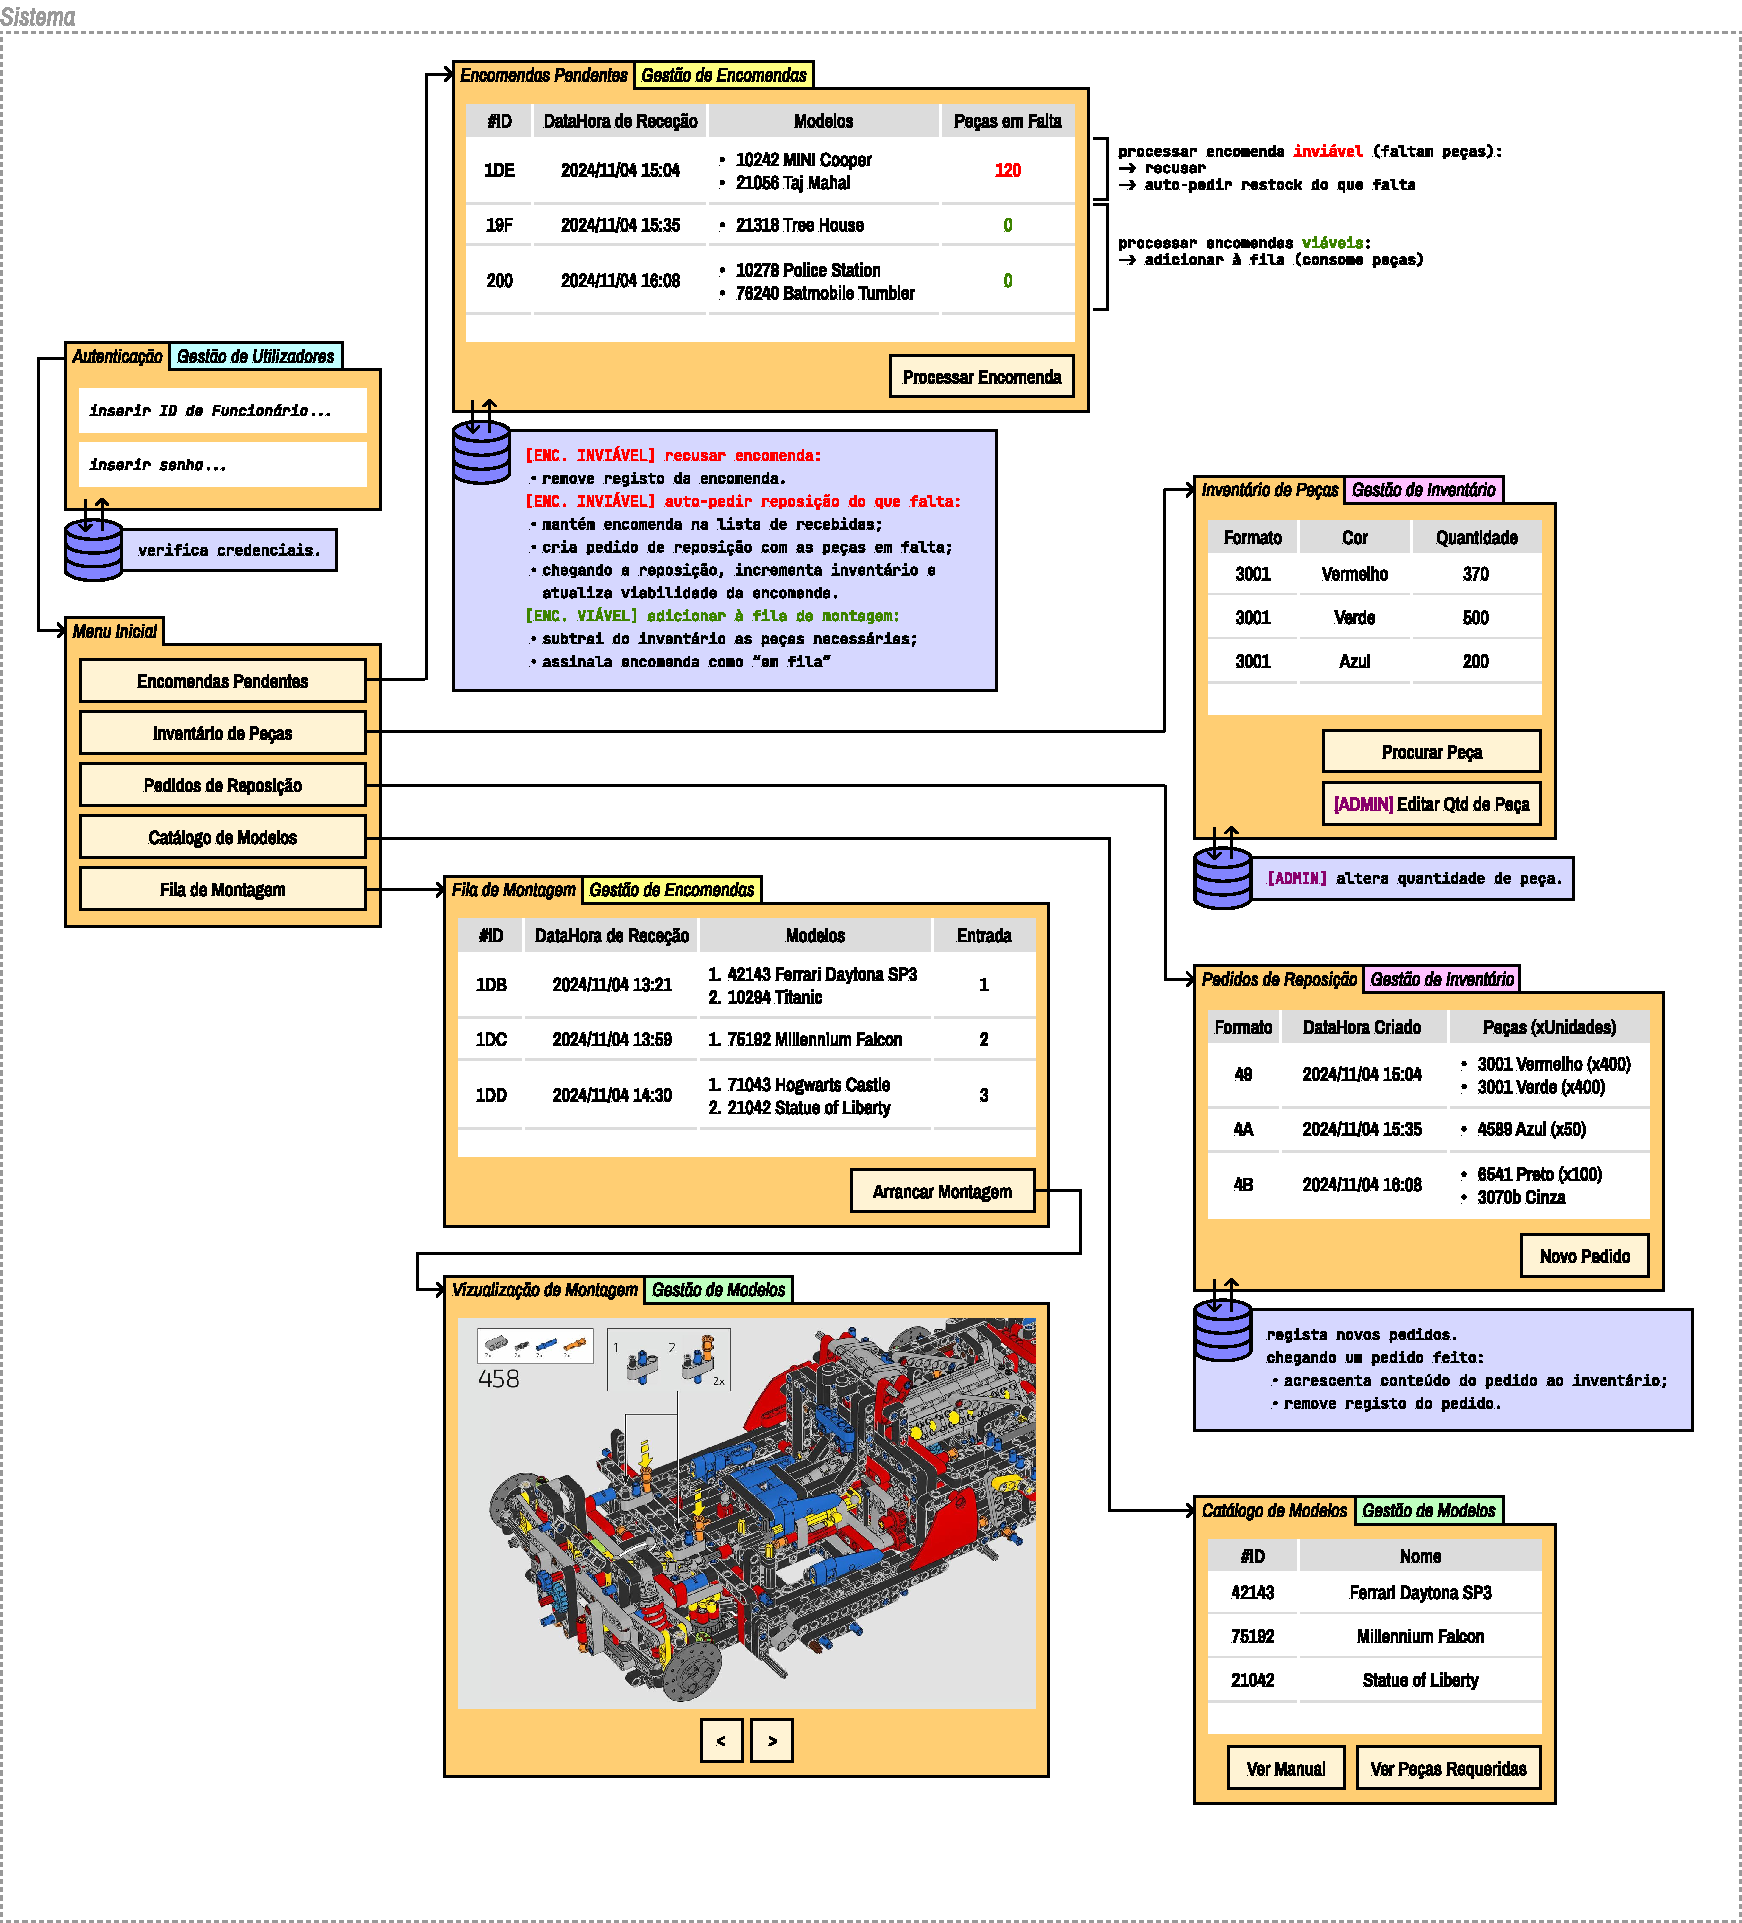
\includegraphics[width=\textwidth]{images/cap1_maquete.pdf}
            \caption{Maquete do sistema.}
            \label{fig:maquete}
        \end{figure}

        
    \newpage
    \section{Métricas de Sucesso}

    O sucesso do sistema pode ser avaliado recorrendo a uma sondagem, posterior à introdução do programa na empresa, segundo os seguintes critérios:
    \begin{enumerate}
        \item Medidas Industriais
            \begin{itemize}
                \item A implementação do sistema contribuiu para aumentar a eficiência da linha de montagem?
                \item Houve um aumento na média de encomendas processadas por dia?
            \end{itemize}
        \item Medidas de Utilização 
            \begin{itemize}
                \item Qual a média de aprovação dos funcionários em relação à adoção do novo sistema?
                \item Quanto tempo foi necessário para os funcionários se habituarem à nova interface?
            \end{itemize}
        \item Medidas Financeiras  
            \begin{itemize}
                \item O sistema causou crescimento significante nos lucros?
                \item Em quanto tempo o sistema conseguiu cobrir o custo inicial de investimento?
                \item Os custos recorrentes de manutenção justificam-se perante os resultados obtidos?
            \end{itemize}
    
    
    \end{enumerate}
     
    \newpage
    \section{Plano de Desenvolvimento}
    
        Com o intuito de preparar e planear o desenvolvimento de todo o projeto, foi delineado um diagrama de Gantt, ilustrado na figura seguinte. A escolha deste tipo de diagrama, deve‐se a vários fatores, entre eles: a clara visualização cronográfica das diversas tarefas, a facilidade de alocação de recursos humanos a cada tarefa e, finalmente, a possibilidade de planeamento a longo prazo.
        
        A localização temporal das várias tarefas no desenvolvimento depende do que requeiram de base. Por exemplo, a modelação requer requisitos, logo a engenharia de requisitos precede a modelação. A modelação estrutural é a base para a definição do sistema de dados, logo esta última vem a seguir.

        Na primeira reunião de equipa, estabeleceu-se a realização de reuniões semanalmente e distribuiram-se tarefas pela primeira vez. Tal distribuição foi sendo modificada à medida que se avançava e tomava melhor ideia do tempo que necessitariam. Deste modo, o planeamento de trabalho tomou a metodologia \textit{agile} como inspiração. 
        
        \begin{figure}[h!]
            \centering
            \includegraphics[width=\textwidth]{images/gantt.png}
            \caption{Diagrama de Gantt}
            \label{Diagrama de Gantt}
        \end{figure}
    

%==========================================================================
% END #1 - INTRO
%==========================================================================